\thispagestyle{empty}
\begin{center}
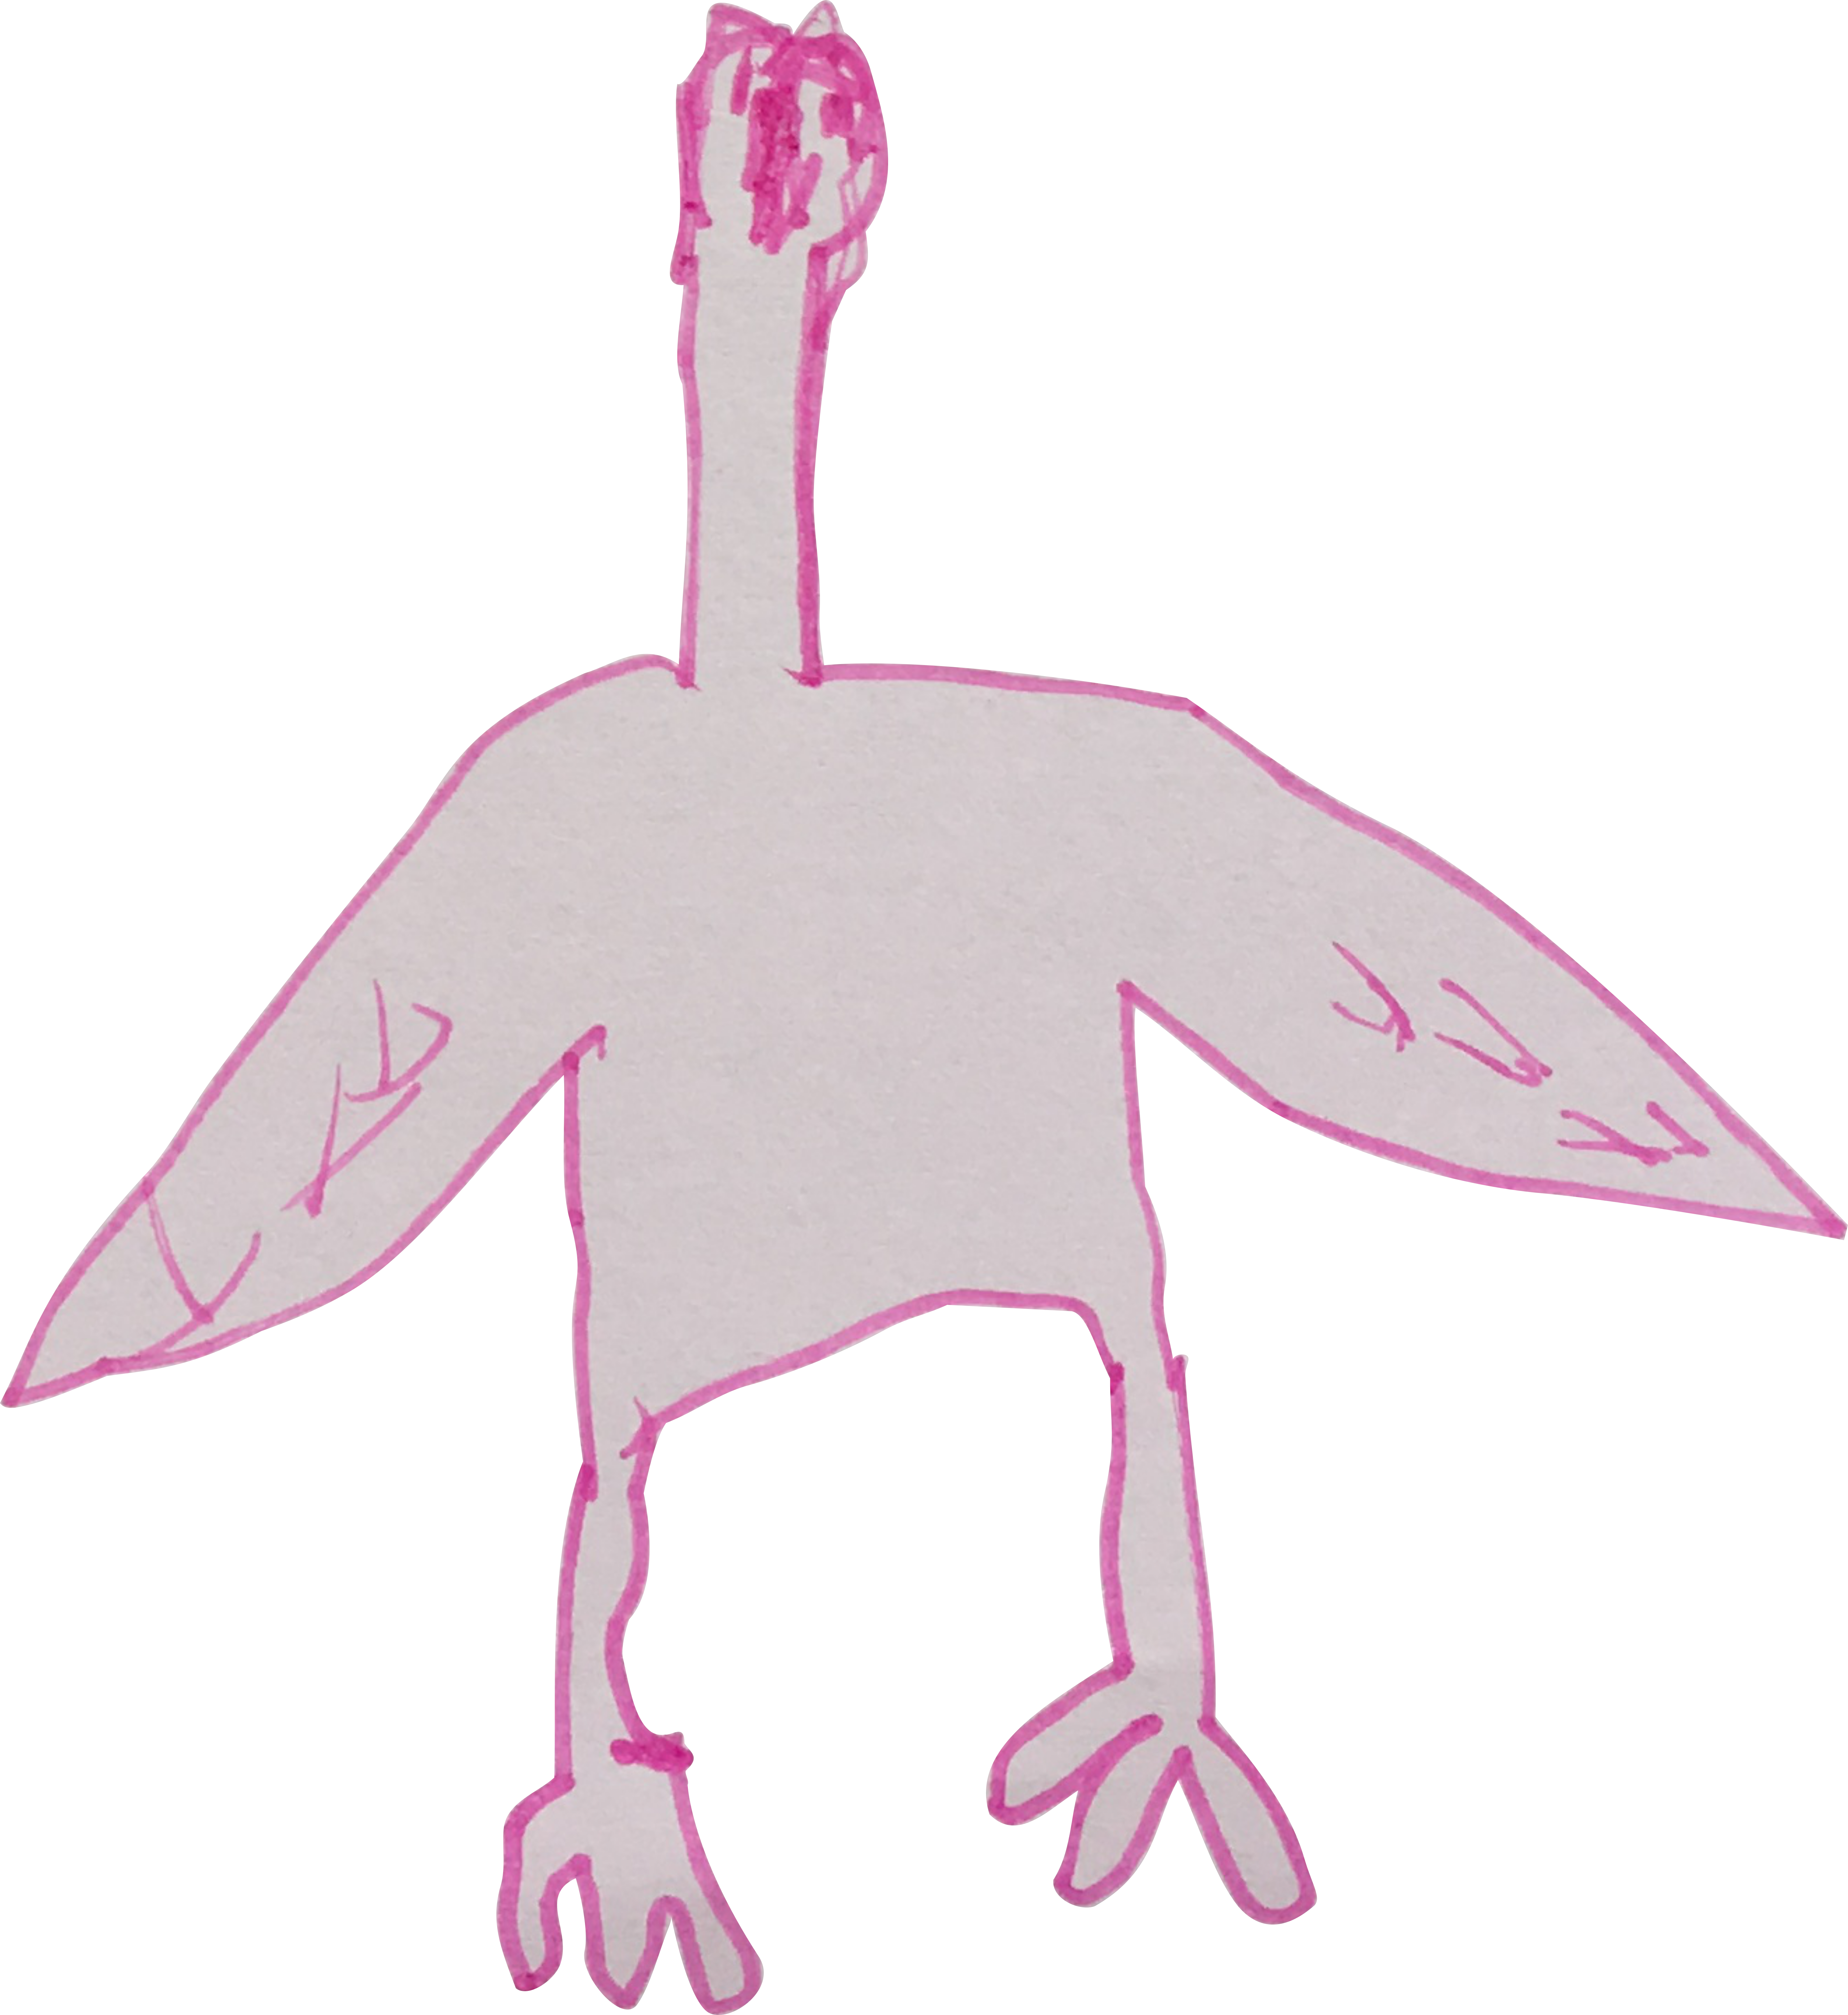
\includegraphics[height=.7\textheight]{./bilder/huhn2.png}
\end{center}
\vskip 2cm
{\Huge\color{farbe}\hfill{\tt{Hühner}}}
\addcontentsline{toc}{chapter}{Hühner}
\newpage
%%%%%%%%%%%%%%%%%%%%%%%%%%%%%%%%%%%%%%%%%%%%%%%%%%%%%%%%%%%%%%%%%%%%%%%%%%%%%%%
\lettrine[lines=2, lhang=.2, loversize=.25, lraise=0.05, findent=0.1em,
nindent=0em]{W}{}ie jeden Sonntagmorgen streiten sich der Hahn Jan und die
Henne Johanna. Die anderen Hühner ziehen sich in solchen Momenten in die
hinterste Ecke des Hühnerhofs zurück und warten bis am Mittag die Bäuerin die
Essenreste bringt, dann ist meisten wieder Ruhe. 

Die Henne Johanna und der Hahn Jahn sind legen sehr viel Wert darauf, gebildet
zu sein und zeigen das auch gerne. Sie können leidenschaftlich ihre Meinung
vertreten, die aber immer genau das Gegenteil der Meinung des anderen ist. 

\enquote{Wenn due so schlau bist wie Du meinst, mein lieber Jan, dann verrate
mir doch mal, was zuerst da war, eine Hehnne oder ein Ei!}

Die Hehnne Johanna weiss natürlich, dass es gar nicht so einfach ist, dieses
Rätsel zu lösen und lächelt spöttisch. Das sieht natürlich niemand, ein Lächeln
zu zeigen, fällt Hühnern im Allgemeinen ziemlich schwer.


\enquote{Ach was für eine uninteressante Frage!} Hahn Jan kratzt auf dem Boden
herum, ob nicht vielleicht doch mal wieder ein Regenwurm in der Nähe ist. 

\enquote{Zuerst meine liebe Johanna, war weder ein Ei, noch eine Henne, sondern natürlich ein Hahn.}

Da die Henne Johanna nicht sofort antwortet, meint Hahn Jan schon, diese Runde
gewonnen zu haben, plustert die Brust und setzt hinzu:


\enquote{Und glaube mir, das waren glückliche Zeiten!}

Natürlich hat die Antwort Henne Johanna etwas überrascht, aber das darf man in
so einer Diskussion keinesfalls zeigen. Das wäre ja noch schöner.

\enquote{Da lachen ja die Hühner!}

Und tatsächlich lacht sie schallend, dass die anderen Hühner vor Schreck ganz
still stehen und die Köpfe ducken.


\enquote{Hähne mein Lieber, sind bekanntermassen die überflüssigsten Wesen.
Ausser über den Hof zu stolzieren und morgens laut zu krähen, seid ihr zu
nichts zu gebrauchen. Ich habe von Hühnerhöfen gehört, da lebt seit
Generationen kein Hahn mehr und es klappt dort trotzdem alles prima.}

Hahn Jan ist beleidigt und pickt sehr energisch auf dem Boden herum, obwohl
dort gar nichts ist. Vor sich hin schimpfend läuft er einmal dem Zaun entlang.


\enquote{Dann beantworte du mir doch mal eine Frage.}

Hahn Jan bringt die Flügel in eine Stellung, die eigentlich nur für
besonderen Gelegenheiten und grossen Feste reserviert ist.


\enquote{Wer war zuerst da, Hühner oder Bauern?}

Darüber hatte die Henne Johanna noch nie nachgedacht. Jetzt ist sie wirklich
still, weil ihr nichts einfällt. 




\enquote{}


\vfill
